% !TeX spellcheck = en
\documentclass[xcolor=table]{beamer}

\usepackage[french,english]{babel}
%\usepackage{fontspec}

%\setmainfont{Junicode}

%\usetheme{CambridgeUS}
\usepackage{hyperref}


%Appendix frames not counted towards total frames
\usepackage{appendixnumberbeamer}
%%%%/!\
% USEFUL BEAMER HELP
%https://www.cpt.univ-mrs.fr/~masson/latex/Beamer-appearance-cheat-sheet.pdf
\setbeamersize{description width=0.47cm}
\setbeamertemplate{headline}{}
\setbeamertemplate{footline}[frame number]{}
\setbeamertemplate{navigation symbols}{}

\usepackage{graphicx}
\usepackage{multirow}


%\usepackage{minted}
\usepackage{hyperref}
\usepackage{tikz}
\usepackage{tikz-qtree}

\usepackage{subcaption}
\usepackage{eso-pic}




%\AtBeginSection[]
%{
%\begin{frame}<beamer>{Outline}
%\tableofcontents[currentsection,hideothersubsections, sectionstyle=show/shaded]
%\end{frame}
%}

%\AtBeginSubsection[]{%
%\begin{frame}{Plan}%
%\small
%\tableofcontents[currentsection,currentsubsection]%
%\end{frame} }


\usetheme{metropolis}

% Metadata
\title{Greening your database of literary corpora}
\subtitle{How to avoid reinventing vocabularies,
  in favor of sustainable, reusable data models}
\author{Jean-Baptiste Camps \and Kelly Christensen}
\institute{École nationale des chartes, PSL}
\date{DH 2025\\Lisbon, 17th July 2025, \textit{Session SP-31}}


\usepackage{amsmath}
\usepackage{tikz}
\usepackage{tikz-qtree}
\usetikzlibrary{patterns,patterns.meta}
\usetikzlibrary{positioning}
\usepackage{multirow}
\usepackage{minted}
\usepackage{adjustbox}
\usepackage{tabularray}

\usepackage{subcaption}

% Citation packages
\usepackage[autostyle]{csquotes}
\usepackage[
    backend=biber,
    % style=numeric-comp,
    natbib=true,
    url=false,
    doi=true,
    eprint=false
]{biblatex}
\addbibresource{inputs/bib.bib}
\nocite{*}
\usepackage{tablefootnote}

\usepackage{acro}
\acsetup{make-links}

% Acronyms
\DeclareAcronym{cidoc}{
	short=CIDOC,
	long=Comité International pour la DOCumentation
}

\DeclareAcronym{crm}{
  short=CRM,
  long=Conceptual Reference Model
}
\DeclareAcronym{frbr}{
  short=FRBR,
  long=Functional Requirements for Bibliographic Records
}

\DeclareAcronym{frbroo}{
  short=FRBR\textsubscript{OO},
  long=Functional Requirements for Bibliographic Records Object-Oriented
}

\DeclareAcronym{lrm}{
  short=LRM,
  long=Library Reference Model
}
\DeclareAcronym{lrmoo}{
  short=LRM\textsubscript{OO},
  long=Library Reference Model Object-Oriented
}
\DeclareAcronym{ifla}{
  short=IFLA,
  long=International Federation of Library Associations
}
\DeclareAcronym{wemi}{
  short=WEMI,
  long=Work-Expression-Manifestation-Item
}

\DeclareAcronym{htr}{
  short=HTR,
  long=Handwritten Text Recognition
}

\DeclareAcronym{tei}{
  short=TEI,
  long=Text Encoding Initiative
}

\DeclareAcronym{fair}{
  short=FAIR,
  long={Findable, Accessible, Interoperable, Reusable}
}

\DeclareAcronym{dts}{
  short=DTS,
  long=Distributed Text Services
}

\DeclareAcronym{iiif}{
  short=IIIF,
  long=International Image Interoperability Framework
}

\DeclareAcronym{ci}{
  short=CI,
  long=Continuous Integration
}

\DeclareAcronym{pypi}{
  short=PyPI,
  long=Python Package Index
}

\DeclareAcronym{sdh}{
    short=SDH,
    long=CRM Semantic Data for Humanities and Social Sciences
}

\DeclareAcronym{dcmi}{
  short=DC,
  long=Dublin Core
}


\AtBeginSection[]
{
\begin{frame}<beamer>{Outline}
\tableofcontents[currentsection,hideothersubsections, sectionstyle=show/shaded]
\end{frame}
}

\setbeamercolor{background canvas}{bg=white}

\begin{document}

\begin{frame}
    \AddToShipoutPictureFG*{
    \AtPageUpperLeft{\put(0,-15){\makebox[0.98\paperwidth][r]{slides: \href{https://enc.hal.science/hal-05059049}{enc.hal.science/hal-05059049}}}}
}

	\maketitle

	\begin{center}
		\vspace*{-3cm}
		\centering
		
\includegraphics[width=0.37\textwidth]{img/logo-enc.png} \hfill
	    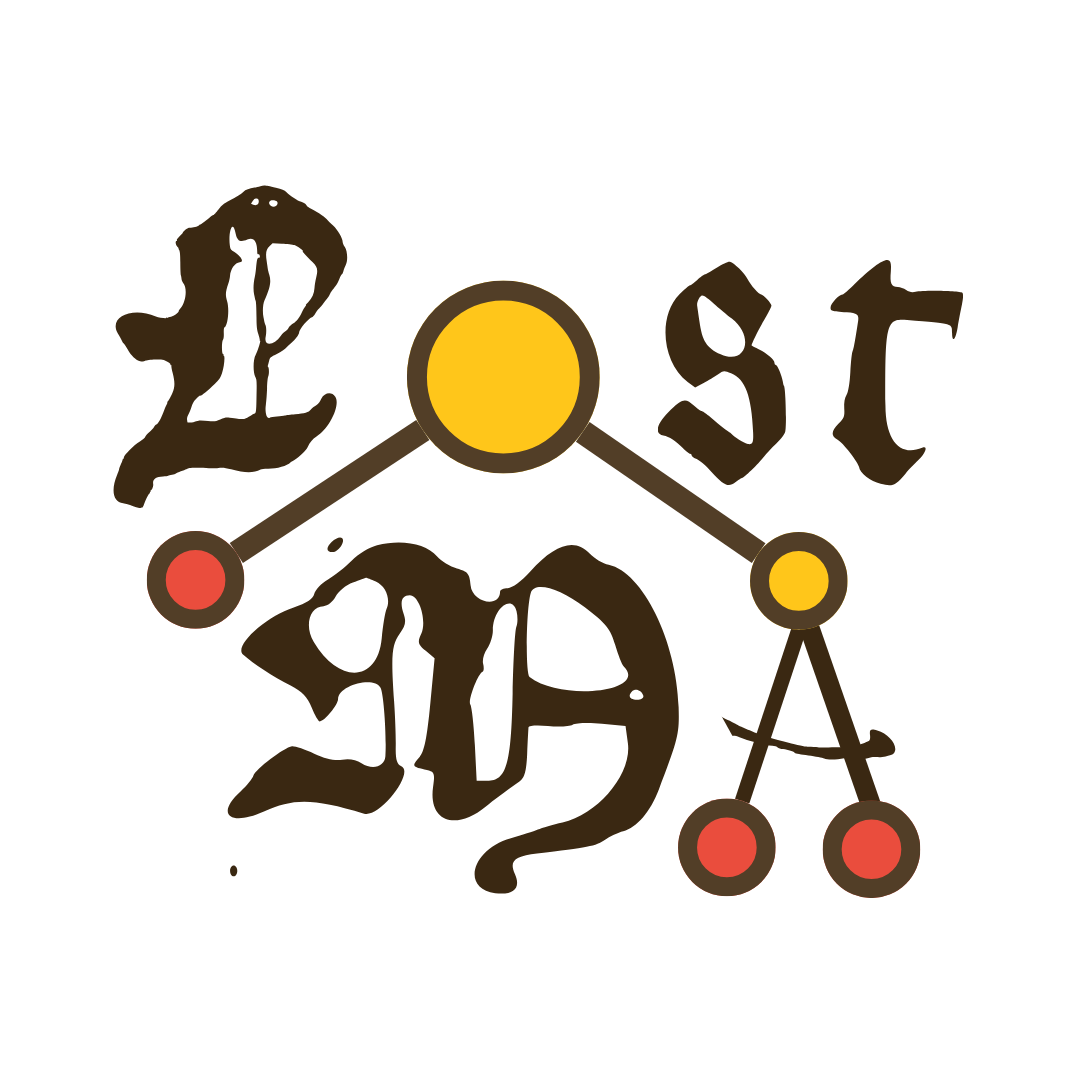
\includegraphics[width=0.15\textwidth]{img/logo_lostma.png} \hfill
	    
\includegraphics[width=0.3\textwidth]{img/logo-erc.png}
	\end{center}

\end{frame}

\begin{frame}{Context: LostMa project}
\AddToShipoutPictureFG*{
    \AtPageUpperLeft{\put(0,-40){\makebox[0.98\paperwidth][r]{slides: \href{https://enc.hal.science/hal-05059049}{enc.hal.science/hal-05059049}}}}
}
\vspace{1em}
\begin{itemize}
    \item Project: \texttt{LostMa}
    \begin{itemize}
        \item European Research Council
        \item 5 years (all good things come to an end)
    \end{itemize}
    \item Goal
        \begin{itemize}
            \item Model the transmission of Medieval stories, texts and manuscripts (and estimate survival rate)
            %\item Train \& evaluate model with variables: narrative content, genre, language, materiality
        \end{itemize}
    \item Problem
        \begin{itemize}
            \item Group manuscripts (easy to distinguish, libraries do this all the time) by narrative content (more abstract, less standardised)
        \end{itemize}
    \item Challenge
        \begin{itemize}
            \item Minimize original ontology. Rely on existing frameworks and digital resources.
            \begin{itemize}
                \item \ac{fair}
            \end{itemize}
        \end{itemize}
\end{itemize}
\end{frame}

\begin{frame}{Problem: Modelling narrative traditions}
What data model makes versions of a story findable (groups them) but also reuses the main bibliographic ontologies?

    \begin{adjustbox}{max totalsize={\textwidth}{0.9\textheight},center}
	\tikzstyle{n} = [circle, minimum width=1.5cm, text width=2cm, text centered, draw=black, fill=gray!10]
\tikzstyle{p} = [rectangle, rounded corners=0.25cm, minimum width=1.5cm, text width=2.25cm, text centered, draw=black, fill=gray!30]

\tikzstyle{arrow} = [thick,->,>=stealth]

\begin{tikzpicture}[-,shorten >=1pt,auto,node distance=0.5cm,semithick]

    \node (text1) [n]
        {Story v.1};%, \\ Chrétien de Troyes \\ (1182-1190)}
    \node (text2) [n, right = of text1, xshift=3cm]
        {Story v.2};%, \\ Wolfram von Eschenbach \\ (1200-1210)}.

    % \draw[<->, dash dot] (story) -- (text1);
    % \draw[<->, dash dot] (story) -- (text2);

    \path[<->, dash dot]
        (text2) edge[bend left=0] (text1);

    \node (conte) [p, below = of text1, xshift=-0.5cm] {\textit{Le conte du graal}};
    \node (troyes) [p, below = of conte] {Chrétien de Troyes};
    \node (fro) [p, below = of troyes] {Old French};

    \node (parzival) [p, below = of text2, xshift=0.5cm] {\textit{Parzival}};
    \node (wolfram) [p, below = of parzival] {Wolfram von Eschenbach};
    \node (gmh) [p, below = of wolfram] {Middle High German};

\end{tikzpicture}
	\end{adjustbox}
\end{frame}

\begin{frame}{Challenge: Reusability and (project) resource management}
    \textit{FAIR Guiding Principles for scientific data management and stewardship} (2016)
    \begin{center}
    \begin{tabular}{|c|c|c|c|} \hline
        F & A & I & R \\
        Findable & Accessible & Interoperable & Reusable \\
        \hline
    \end{tabular}
    \end{center}
    \begin{itemize}
        \item Greener digital data storage and distribution\footfullcite{Ficher2021}
        \item Minimal single-use documentation
        \item Efficient integration in other projects
    \end{itemize}
\end{frame}


\begin{frame}{Methodology: Models for F.A.I.R. literary projects}
    The big groups:
        \begin{itemize}
            \item \acf{cidoc}
            \item \acf{ifla}
            \item \acf{dcmi}
        \end{itemize}
    The main ontologies:
    \begin{table}
    \centering \footnotesize
        \begin{tabular}{|c|c|c|p{0.6\textwidth}|}
            \hline
            \cellcolor{gray!50}\textbf{Org.}
                & \cellcolor{gray!50}\textbf{Year}
                & \cellcolor{gray!50}\textbf{Ver.}
                & \cellcolor{gray!50}\textbf{Model}
                \\ \hline \hline
            \ac{ifla} & 1998 & 1.0 & \ac{frbr}
                \\ \hline
            \cellcolor{gray!10}\ac{cidoc}
                & \cellcolor{gray!10}2006
                & \cellcolor{gray!10}1.0
                & \cellcolor{gray!10}\ac{crm}
                \\ \hline
            \ac{ifla} & 2016 & 2.4 & \ac{frbroo}
                \\ \hline
            \cellcolor{gray!10} \ac{ifla}
                & \cellcolor{gray!10}2017
                & \cellcolor{gray!10}1.0
                & \cellcolor{gray!10}\ac{lrm}
                \\ \hline
            \ac{cidoc} & 2022 & 7.1.12 & \ac{crm}
                \\ \hline
            \cellcolor{yellow!30}\ac{ifla}
                & \cellcolor{yellow!30}2024
                & \cellcolor{yellow!30}1.0
                & \cellcolor{yellow!30}\ac{lrmoo}
                \\ \hline
        \end{tabular}
    \caption{Version release dates of international standards}
    \end{table}
\end{frame}

\begin{frame}{\acf{lrmoo}, built atop the \ac{crm}}
    \begin{adjustbox}{max totalsize={\textwidth}{0.9\textheight},center}
	
\tikzstyle{o} = [circle, minimum width=1.25cm, text width=1.25cm, text centered, draw=black, fill=yellow!30]
\tikzstyle{c} = [circle, minimum width=1cm, text width=1cm, text centered, draw=black,
pattern={north east lines},pattern color=gray!50
]
\tikzstyle{n} = [circle, minimum width=1.25cm, text width=1.25cm, text centered, draw=black, fill=yellow!30]
\tikzstyle{arrow} = [thick,->,>=stealth]

\begin{tikzpicture}[-,shorten >=1pt,auto,node distance=0.15cm,semithick]

    \tiny

    \node (entity) [o]
        {\href{http://www.cidoc-crm.org/cidoc-crm/E1_CRM_Entity}{crm:E1} \textbf{CRM Entity}};

    \node (place) [n, above = of entity, xshift=1.25cm, yshift=0.5cm]
        {\href{http://www.cidoc-crm.org/cidoc-crm/E53_Place}{crm:E53} \textbf{Place}};

    \node (spacetimeVolume) [c, below = of entity, xshift=1.25cm]
        {\href{http://www.cidoc-crm.org/cidoc-crm/E92_Spacetime_Volume}{crm:E92}};
    \node (physicalThing) [o, below = of spacetimeVolume, xshift=1.25cm]
        {\href{http://www.cidoc-crm.org/cidoc-crm/E18_Physical_Thing}{crm:E18} \textbf{Physical Thing}};
    \node (physicalObject) [o, below = of physicalThing, xshift=-1.25cm]
        {\href{http://www.cidoc-crm.org/cidoc-crm/E19_Physical_Object}{crm:E19} \textbf{Physical Object}};
    \node (manMadeObject) [n, below = of physicalObject]
        {\href{http://www.cidoc-crm.org/cidoc-crm/E22_Human-Made_Object}{crm:E22} \textbf{Human-Made Object}};

    \node (persistentItem) [c, right = of entity, xshift=0.5cm]
        {\href{http://www.cidoc-crm.org/cidoc-crm/E77_Persistent_Item}{crm:E77}};
    \node (thing) [o, right = of persistentItem]
        {\href{http://www.cidoc-crm.org/cidoc-crm/E70_Thing}{crm:E70} \textbf{Thing}};
    \node (manMadeThing) [c, right = of thing]
        {\href{http://www.cidoc-crm.org/cidoc-crm/E71_Human-Made_Thing}{crm:E71}};
    \node (conceptualObject) [n, right = of manMadeThing]
        {\href{http://www.cidoc-crm.org/cidoc-crm/E28_Conceptual_Object}{crm:E28} \textbf{Conceptual Object}};

    \node (propositionalObject) [o, right = of conceptualObject]
        {\href{http://www.cidoc-crm.org/cidoc-crm/E89_Propositional_Object}{crm:E89} \textbf{Propositional Object}};
    \node (work) [n, right = of propositionalObject, yshift=1.25cm]
        {\href{http://iflastandards.info/ns/lrm/lrmoo/F1_Work}{lrmoo:F1} \textbf{Work}};

    \node (informationObject) [o, right = of propositionalObject, yshift=-1.25cm]
        {\href{http://www.cidoc-crm.org/cidoc-crm/E73_Information_Object}{cmr:E73} \textbf{Information Object}};
    \node (expression) [n, below = of informationObject, xshift=-1.7cm, yshift=-1cm]
        {\href{http://iflastandards.info/ns/lrm/lrmoo/F2_Expression}{lrmoo:F2} \textbf{Expression}};
    \node (manifestation) [n, below = of informationObject, yshift=-3cm]
        {\href{http://iflastandards.info/ns/lrm/lrmoo/F3_Manifestation}{lrmoo:F3} \textbf{Manifestation}};

    \node (physicalManMadeThing) [o, below = of physicalThing, xshift=1.25cm]
        {\href{http://www.cidoc-crm.org/cidoc-crm/E24_Physical_Human-Made_Thing}{crm:E24} \textbf{Physical Human-Made Thing}};
    \node (item) [n, below = of physicalManMadeThing]
        {\href{http://iflastandards.info/ns/lrm/lrmoo/F5_Item}{lrmoo:F5} \textbf{Item}};

    \draw (manMadeThing) -- (conceptualObject);
    \draw (manMadeThing) -- (physicalManMadeThing);
    \draw (physicalManMadeThing) -- (manMadeObject);
    \draw (conceptualObject) -- (propositionalObject);
    \draw (propositionalObject) -- (informationObject);
    \draw (propositionalObject) -- (work);
    \draw (informationObject) -- (manifestation);
    \draw (informationObject) -- (expression);
    \draw (physicalManMadeThing) -- (item);
    \draw (manMadeThing) -- (thing);
    \draw (thing) -- (persistentItem);
    \draw (entity) -- (persistentItem);

    \draw (entity) -- (place);

    \draw (entity) -- (spacetimeVolume);
    \draw (spacetimeVolume) -- (physicalThing);
    \draw (physicalThing) -- (physicalManMadeThing);
    \draw (physicalThing) -- (physicalObject);
    \draw (physicalObject) -- (manMadeObject);

    \draw[-, dash dot]
        (place) edge[bend right=20]
        node[left, yshift=-0.5cm]
        {\href{http://www.cidoc-crm.org/cidoc-crm/P55_has_current_location}{crm:P55}}
        node[left, yshift=-0.7cm]
        {CurrentlyHolds}
        (physicalObject)
        ;

    \draw[->, dash dot]
        (physicalThing.30) arc (-60:170:4mm)
        node[above, xshift=0.4cm, yshift=0.4cm]
        {\href{http://www.cidoc-crm.org/cidoc-crm/P46i_forms_part_of}{crm:P46}}
        node [above, xshift=0.4cm, yshift=0.6cm] {FormsPartOf}
        ;

    \draw[->, dash dot]
        (work.30) arc (-60:170:4mm)
        node[below, xshift=0.5cm, yshift=0.9cm]
        {\href{http://iflastandards.info/ns/lrm/lrmoo/R2_is_derivative_of}{lrmoo:R2}}
        node [below, xshift=0.75cm, yshift=0.7cm]
        {IsDerivativeOf}
        ;

    \draw[-, dash dot]
        (work) edge[bend right=30]
        node[above, yshift=0.3cm]
        {\href{http://iflastandards.info/ns/lrm/lrmoo/R10_is_member_of}{lrmoo:R10}}
        node[above, yshift=0.1cm]
        {IsMemberOf}
        (conceptualObject);

    \draw[-, dash dot]
        (work) edge[bend left=60]
        node[right]
        {\href{http://iflastandards.info/ns/lrm/lrmoo/R3_is_realised_in}{lrmoo:R3}}
        node[right, yshift=-0.2cm]{Realises}
        (expression);

    \draw[->, dash dot]
        (expression.-45) arc (60:-190:4mm)
        node[left, yshift=-0.2cm]
        {\href{http://iflastandards.info/ns/lrm/lrmoo/R76_is_derivative_of}{lrmoo:R76}}
        node [left, yshift=-0.4cm]
        {IsDerivativeOf}
        ;

    \draw[-, dash dot]
        (expression) edge[bend left=30] node[right, yshift=0.2cm]
        {\href{http://iflastandards.info/ns/lrm/lrmoo/R4i_is_embodied_in}{lrmoo:R4}}
        node[right] {Embodies}
        (manifestation);

    \draw[-, dash dot]
        (manifestation) edge[bend left=30]
        node[right, xshift=-0.2cm, yshift=-0.2cm]
            {
            \href{http://iflastandards.info/ns/lrm/lrmoo/R7i_is_exemplified_by}
            {lrmoo:R7}}
        node[right, xshift=-0.2cm, yshift=-0.4cm]
            {Exemplifies}
        (item);

\end{tikzpicture}
	\end{adjustbox}
\end{frame}

\begin{frame}{LostMa Ontology, built atop the \ac{lrmoo}}
    \begin{adjustbox}{max totalsize={\textwidth}{0.9\textheight},center}
	\tikzstyle{c} = [circle, minimum width=1cm, text width=1cm, text centered, draw=black!30,
pattern={north east lines},pattern color=gray!50
]
\tikzstyle{n} = [circle, minimum width=1.25cm, text width=1.3cm, text centered, draw=black, fill=yellow!30]
\tikzstyle{p} = [circle, minimum width=1.25cm, text width=1.3cm, text centered, draw=black, fill=yellow!80]

\tikzstyle{arrow} = [thick,->,>=stealth]

\begin{tikzpicture}[-,shorten >=1pt,auto,node distance=0.15cm,semithick]

    \tiny

    \node (entity) [c]
        {\href{http://www.cidoc-crm.org/cidoc-crm/E1_CRM_Entity}{crm:E1}};

    \node (place) [p, above = of entity, xshift=1.25cm, yshift=0.5cm]
        {\href{http://www.cidoc-crm.org/cidoc-crm/E53_Place}{crm:E53} \textbf{Place} / \textbf{Repository}};

    \node (spacetimeVolume) [c, below = of entity, xshift=1.25cm]
        {\href{http://www.cidoc-crm.org/cidoc-crm/E92_Spacetime_Volume}{crm:E92}};
    \node (physicalThing) [c, below = of spacetimeVolume, xshift=1.25cm]
        {\href{http://www.cidoc-crm.org/cidoc-crm/E18_Physical_Thing}{crm:E18} Physical Thing};
    \node (physicalObject) [c, below = of physicalThing, xshift=-1.25cm]
        {\href{http://www.cidoc-crm.org/cidoc-crm/E19_Physical_Object}{crm:E19}};
    \node (document) [p, below = of physicalObject]
        {\href{http://www.cidoc-crm.org/cidoc-crm/E22_Human-Made_Object}{crm:E22} \textbf{Document}};

    \node (persistentItem) [c, right = of entity, xshift=0.5cm]
        {\href{http://www.cidoc-crm.org/cidoc-crm/E77_Persistent_Item}{crm:E77}};
    \node (thing) [c, right = of persistentItem, xshift=0.2cm]
        {\href{http://www.cidoc-crm.org/cidoc-crm/E70_Thing}{crm:E70}};
    \node (manMadeThing) [c, right = of thing]
        {\href{http://www.cidoc-crm.org/cidoc-crm/E71_Human-Made_Thing}{crm:E71} Human-Made Thing};
    \node (storyverse) [n, right = of manMadeThing]
        {\href{http://www.cidoc-crm.org/cidoc-crm/E28_Conceptual_Object}{crm:E28} Concept. Object / \textbf{Storyverse}};

    \node (propositionalObject) [c, right = of storyverse]
        {\href{http://www.cidoc-crm.org/cidoc-crm/E89_Propositional_Object}{crm:E89} Prop. Object};
    \node (story) [n, right = of propositionalObject, yshift=1.25cm]
        {\href{http://iflastandards.info/ns/lrm/lrmoo/F1_Work}{lrmoo:F1} \textbf{Story}};

    \node (informationObject) [c, right = of propositionalObject, yshift=-1.25cm]
        {\href{http://www.cidoc-crm.org/cidoc-crm/E73_Information_Object}{cmr:E73} Info. Object};
    \node (text) [n, below = of informationObject, xshift=-1.7cm, yshift=-1cm]
        {\href{http://iflastandards.info/ns/lrm/lrmoo/F2_Expression}{lrmoo:F2} \textbf{Text}};
    \node (witness) [n, below = of informationObject, yshift=-3cm]
        {\href{http://iflastandards.info/ns/lrm/lrmoo/F3_Manifestation}{lrmoo:F3} \textbf{Witness}};

    \node (physicalManMadeThing) [c, below = of physicalThing, xshift=1.25cm]
        {\href{http://www.cidoc-crm.org/cidoc-crm/E24_Physical_Human-Made_Thing}{crm:E24}};
    \node (part) [n, below = of physicalManMadeThing]
        {\href{http://iflastandards.info/ns/lrm/lrmoo/F5_Item}{lrmoo:F5} \textbf{Part}};

    \draw (manMadeThing) -- (storyverse);
    \draw (manMadeThing) -- (physicalManMadeThing);
    \draw (physicalManMadeThing) -- (document);
    \draw (storyverse) -- (propositionalObject);
    \draw (propositionalObject) -- (informationObject);
    \draw (propositionalObject) -- (story);
    \draw (informationObject) -- (witness);
    \draw (informationObject) -- (text);
    \draw (physicalManMadeThing) -- (part);
    \draw (manMadeThing) -- (thing);
    \draw (thing) -- (persistentItem);
    \draw (entity) -- (persistentItem);

    \draw (entity) -- (place);

    \draw (entity) -- (spacetimeVolume);
    \draw (spacetimeVolume) -- (physicalThing);
    \draw (physicalThing) -- (physicalManMadeThing);
    \draw (physicalThing) -- (physicalObject);
    \draw (physicalObject) -- (document);

    \draw[->, dash dot, line width=1.5pt]
        (document) edge[bend left=20]
        node[left, yshift=-0.5cm]
        {\href{http://www.cidoc-crm.org/cidoc-crm/P55_has_current_location}{crm:P55}}
        node[left, yshift=-0.7cm]
        {HasCurrentLocation}
        (place)
        ;

    \draw[->, dash dot, line width=1.5pt]
        (part) edge [bend left=45]
        node[below, yshift=-0.1cm]
        {\href{http://www.cidoc-crm.org/cidoc-crm/P46i_forms_part_of}{crm:P46}}
        node [below, yshift=-0.3cm] {FormsPartOf}
        (document)
        ;

    \draw[->, dash dot, line width=1.5pt]
        (story.30) arc (-60:170:4mm)
        node[below, xshift=0.5cm, yshift=0.9cm]
        {\href{http://iflastandards.info/ns/lrm/lrmoo/R2_is_derivative_of}{lrmoo:R2}}
        node [below, xshift=0.75cm, yshift=0.7cm]
        {IsDerivativeOf}
        ;

    \draw[->, dash dot, line width=1.5pt]
        (story) edge[bend right=30]
        node[above, yshift=0.3cm]
        {\href{http://iflastandards.info/ns/lrm/lrmoo/R10_is_member_of}{lrmoo:R10}}
        node[above, yshift=0.1cm]
        {IsMemberOf}
        (storyverse);

    \draw[->, dash dot, line width=1.5pt]
        (story) edge[bend left=60]
        node[right]
        {\href{http://iflastandards.info/ns/lrm/lrmoo/R3_is_realised_in}{lrmoo:R3}}
        node[right, yshift=-0.2cm]{IsRealisedIn}
        (text);

    \draw[->, dash dot, line width=1.5pt]
        (text.-45) arc (60:-190:4mm)
        node[left, yshift=-0.2cm]
        {\href{http://iflastandards.info/ns/lrm/lrmoo/R76_is_derivative_of}{lrmoo:R76}}
        node [left, yshift=-0.4cm]
        {IsDerivativeOf}
        ;

    \draw[->, dash dot, line width=1.5pt]
        (text) edge[bend left=30] node[right, yshift=0.2cm]
        {\href{http://iflastandards.info/ns/lrm/lrmoo/R4i_is_embodied_in}{lrmoo:R4}}
        node[right] {IsEmbodiedIn}
        (witness);

    \draw[->, dash dot, line width=1.5pt]
        (witness) edge[bend left=30]
        node[right, xshift=-0.2cm, yshift=-0.2cm]
            {
            \href{http://iflastandards.info/ns/lrm/lrmoo/R7i_is_exemplified_by}
            {lrmoo:R7}}
        node[right, xshift=-0.2cm, yshift=-0.4cm]
            {IsExemplifiedBy}
        (part);

\end{tikzpicture}
	\end{adjustbox}
\end{frame}

\begin{frame}{LostMa Ontology, simplified}
    \begin{adjustbox}{max totalsize={\textwidth}{0.9\textheight},center}
	\tikzstyle{n} = [circle, minimum width=1.5cm, text width=1.5cm, text centered, draw=black, fill=yellow!30]
\tikzstyle{p} = [circle, minimum width=1.5cm, text width=1.5cm, text centered, draw=black, fill=yellow!80]

\tikzstyle{arrow} = [thick,->,>=stealth]

\begin{tikzpicture}[-,shorten >=1pt,auto,node distance=0.15cm,semithick]

    \scriptsize

    \node (storyverse) [n]
        {\href{http://www.cidoc-crm.org/cidoc-crm/E28_Conceptual_Object}{crm:E28} \textbf{Storyverse}};

    \node (story) [n, right = of storyverse]
        {\href{http://iflastandards.info/ns/lrm/lrmoo/F1_Work}{lrmoo:F1} \textbf{Story}};

    \node (text) [n, right = of story]
        {\href{http://iflastandards.info/ns/lrm/lrmoo/F2_Expression}{lrmoo:F2} \textbf{Text}};

    \node (witness) [n, right = of text]
        {\href{http://iflastandards.info/ns/lrm/lrmoo/F3_Manifestation}{lrmoo:F3} \textbf{Witness}};

    \node (part) [n, right = of witness]
        {\href{http://iflastandards.info/ns/lrm/lrmoo/F5_Item}{lrmoo:F5} \textbf{Part}};

    \node (document) [p, below = of part, yshift=-1cm]
        {\href{http://www.cidoc-crm.org/cidoc-crm/E22_Human-Made_Object}{crm:E22} \textbf{Document}};

    \node (repository) [p, left = of document]
        {\href{http://www.cidoc-crm.org/cidoc-crm/E53_Place}{crm:E53} \textbf{Repository}};

    \draw[->, line width=1pt]
        (document) edge[bend left=90]
        node[below]
        {\href{http://www.cidoc-crm.org/cidoc-crm/P55_has_current_location}{crm:P55}}
        node[below, yshift=-0.4cm]
        {HasCurrentLocation}
        (repository)
        ;

    \draw[->, line width=1pt]
        (part) edge [bend left=0]
        node[right, yshift=0.2cm]
        {\href{http://www.cidoc-crm.org/cidoc-crm/P46i_forms_part_of}{crm:P46}}
        node [right, yshift=-0.2cm] {FormsPartOf}
        (document)
        ;

    \draw[->, line width=1.5pt]
        (story.-45) arc (60:-190:4mm)
        node[below, yshift=-0.5cm]
        {\href{http://iflastandards.info/ns/lrm/lrmoo/R2_is_derivative_of}{lrmoo:\textbf{R2}}}
        node [below, yshift=-0.9cm]
        {IsDerivativeOf}
        ;

    \path[->, line width=1.5pt]
        (story.north) edge[bend right=90]
        node[above, yshift=0.4cm]
        {\href{http://iflastandards.info/ns/lrm/lrmoo/R10_is_member_of}{lrmoo:\textbf{R10}}}
        node[above]
        {IsMemberOf}
        (storyverse.north);

    \path[<-, line width=1.5pt]
        (story.80) edge[bend left=90]
        node[above, yshift=0.4cm]
        {\href{http://iflastandards.info/ns/lrm/lrmoo/R3_is_realised_in}{lrmoo:\textbf{R3}}}
        node[above]{Realises}
        (text.north);

    \draw[->, line width=1.5pt]
        (text.-45) arc (60:-190:4mm)
        node[below, yshift=-0.5cm]
        {\href{http://iflastandards.info/ns/lrm/lrmoo/R76_is_derivative_of}{lrmoo:\textbf{R76}}}
        node [below, yshift=-0.9cm]
        {IsDerivativeOf}
        ;

    \path[<-, line width=1.5pt]
        (text.80) edge[bend left=90] node[above, yshift=0.4cm]
        {\href{http://iflastandards.info/ns/lrm/lrmoo/R4i_is_embodied_in}{lrmoo:\textbf{R4}}}
        node[above] {Embodies}
        (witness.north);

    \path[->, line width=1.5pt]
        (witness.north) edge[bend left=90]
        node[above, yshift=0.4cm]
            {
            \href{http://iflastandards.info/ns/lrm/lrmoo/R7i_is_exemplified_by}
            {lrmoo:\textbf{R7}}}
        node[above]
            {IsExemplifiedBy}
        (part.north);

\end{tikzpicture}
	\end{adjustbox}
\end{frame}

\begin{frame}{Solution: Perceval example (revisited)}
    \begin{adjustbox}{max totalsize={\textwidth}{0.9\textheight},center}
	\tikzstyle{n} = [circle, minimum width=1.5cm, text width=2cm, text centered, draw=black, fill=gray!10]
\tikzstyle{p} = [rectangle, rounded corners=0.25cm, minimum width=1.5cm, text width=2.25cm, text centered, draw=black, fill=gray!30]

\tikzstyle{arrow} = [thick,->,>=stealth]

\begin{tikzpicture}[-,shorten >=1pt,auto,node distance=0.5cm,semithick]

    \node (story) [n] {Story};

    \node (perceval) [p, right = of story, xshift=1.5cm] {Perceval};
    \draw[->] (story) --
    node [above]{\href{http://purl.org/dc/terms/title}{dcterms:title}}
    (perceval);

    \node (text1) [n, left = of story, yshift=-2.5cm, xshift=-1cm]
        {Text 1};%, \\ Chrétien de Troyes \\ (1182-1190)}
    \node (text2) [n, right = of story, yshift=-2.5cm, xshift=1cm]
        {Text 2};%, \\ Wolfram von Eschenbach \\ (1200-1210)}.

    \draw[->, line width=2pt] (story) --
        node[above, xshift=-0.6cm]
            {\href{http://iflastandards.info/ns/lrm/lrmoo/R3_is_realised_in}{lrmoo:R3}}
        (text1);
    \draw[->, line width=2pt] (story) --
        node[above, xshift=1.3cm]{
            \href{http://iflastandards.info/ns/lrm/lrmoo/R3_is_realised_in}{lrmoo:R3}
            \footnotesize{IsRealisedIn}
        }
        (text2);

    \path[->, line width=2pt]
        (text2) edge[bend left=0]
        node[above]
        {\href{http://iflastandards.info/ns/lrm/lrmoo/R76_is_derivative_of}{lrmoo:R76}}
        node[below]{\footnotesize{IsDerivativeOf}}
        (text1);

    \node (conte) [p, below = of text1, yshift=-0.25cm, xshift=-0.5cm] {\textit{Le conte du graal}};
    \node (troyes) [p, below = of conte] {Chrétien de Troyes};
    \node (fro) [p, below = of troyes] {Old French};

    \node (parzival) [p, below = of text2, yshift=-0.25cm, xshift=0.5cm] {\textit{Parzival}};
    \node (wolfram) [p, below = of parzival] {Wolfram von Eschenbach};
    \node (gmh) [p, below = of wolfram] {Middle High German};

    \path[->]
        (text1) edge[bend left=0]
        node [right]
        {\href{http://purl.org/dc/terms/title}
        {dcterms:title}}
        (conte);
    \path[->]
        (text1.east) edge[bend left=45]
        node [right, text width=1cm]
        {\href{http://purl.org/dc/terms/language}
        {dcterms:language}}
        (fro.east);
    \path[->]
        (text1.west) edge[bend right=60]
        node [left, yshift=1cm, xshift=1.75cm]
        {\href{http://purl.org/dc/terms/creator}
        {dcterms:creator}}
        (troyes.west);

    \path[->]
        (text2) edge[bend right=0]
        node [right]
        {\href{http://purl.org/dc/terms/title}
        {dcterms:title}}
        (parzival);
    \path[->]
        (text2.east) edge[bend left=45]
        node [below, xshift=0.4cm]
        {\href{http://purl.org/dc/terms/language}
        {dcterms:language}}
        (gmh.east);
    \path[->]
        (text2.west) edge[bend right=60]
        node [left, xshift=1cm]
        {\href{http://purl.org/dc/terms/creator}
        {dcterms:creator}}
        (wolfram.west);

\end{tikzpicture}
	\end{adjustbox}
\end{frame}

\begin{frame}[containsverbatim]{Solution: Multi-use documentation (text)}
Namespaces:
    \texttt{\href{http://iflastandards.info/ns/lrm/lrmoo}{lrmoo}} (IFLA),
    \texttt{\href{http://purl.org/dc/terms/1.1}{dcterms}} (DCMI),
    \texttt{\href{http://purl.org/dc/elements/1.1}{dc}} (DCMI)
\begin{minted}{xml}
<lrmoo:F2_Expression id="48572">
 <dcterms:title>Perceval</dcterms:title>
 <dcterms:language>fro</dcterms:language>
 <dcterms:created>1196-01-01/1210-12-31</dcterms:created>
 <dc:date>Vers 1200</dc:date>
 <lrmoo:R4_is_embodied_in>
  <lrmoo:F3_Manifestation id="54725">
   <!-- Witness metadata -->
 </lrmoo:R4_is_embodied_in>
</lrmoo:F2_Expression>
\end{minted}
\end{frame}

\begin{frame}[containsverbatim]{Solution: Multi-use documentation (witness)}
Namespaces:
  \texttt{\href{http://iflastandards.info/ns/lrm/lrmoo}{lrmoo}} (IFLA),
    \texttt{\href{http://purl.org/dc/terms/1.1}{dcterms}} (DCMI),
    \texttt{\href{http://www.cidoc-crm.org/cidoc-crm}{crm}} (CIDOC),
    \texttt{\href{http://purl.org/ontology/bibo}{bibo}} (DCMI)
\scriptsize
\begin{minted}{xml}
<lrmoo:F3_Manifestation id="54725">
 <dcterms:created>1301-01-01/1400-12-31</dcterms:created>
 <lrmoo:R7_is_exemplified_by>
  <lrmoo:F5_Item id="53068">
   <bibo:locator>
    <bibo:pages>
     <bibo:pageStart>96r</bibo:pageStart>
     <bibo:pageEnd>126v</bibo:pageEnd>
    </bibo:pages>
   </bibo:locator>
   <crm:P46i_forms_part_of>
    <crm:E22_Human-Made_Object id="46077"/>
     <!-- Document metadata -->
   </crm:P46i_forms_part_of>
  </lrmoo:F5_Item>
 </lrmoo:R7_is_exemplified_by>
</lrmoo:F3_Manifestation>
\end{minted}
\end{frame}

\begin{frame}{Conclusion}

\AddToShipoutPictureFG*{
    \AtPageUpperLeft{\put(0,-40){\makebox[0.98\paperwidth][r]{slides: \href{https://enc.hal.science/hal-05059049}{enc.hal.science/hal-05059049}}}}
}

\vspace{1em}
\begin{block}{In progress}
    \begin{itemize}
        \item Off-load documentation of our data model to existent digital resources by linking our ontology to others' documentation
        \begin{itemize}
            \item Side goal: save on resources for maintaining online documentation (esp. after project ends)
        \end{itemize}
        \item Map more properties to our core (\ac{lrmoo}, \ac{crm}) entities
    \end{itemize}
\end{block}
\begin{block}{Future work}
    \begin{itemize}
        \item Accommodate more uncertainty in values, i.e. dates:
        \begin{itemize}
            \item earliest possible date
            \item estimated earliest date
            \item estimated latest date
            \item latest possible date
        \end{itemize}
        \item Accommodate source citation on properties
    \end{itemize}
\end{block}
\end{frame}


\end{document}